\chapter{Background}

\section{Parallel Computing}

\subsection{Definition}

As the name imply, parallel computing is about executing task simultaneously based on the given computer resource to find a solution to a complex computational problem, such as modeling and simulation. Unlike the traditional serial computation, where instructions are executed in succession one at a time, in parallelization, a problem are separated many different, disctint segments, each segment can be further decomposed into set of instructions. The distintion between these segments allows them to be performed on different processors in parallel fashion. The computation resource required for parallel computing, as stated previously, can be either a powerful computer with a multiple cores/threads CPU or a network of serveral computers, with or without dedicated GPUs. \\
%Images represent serial and parallel computing
~\\
\begin{figure}[H]
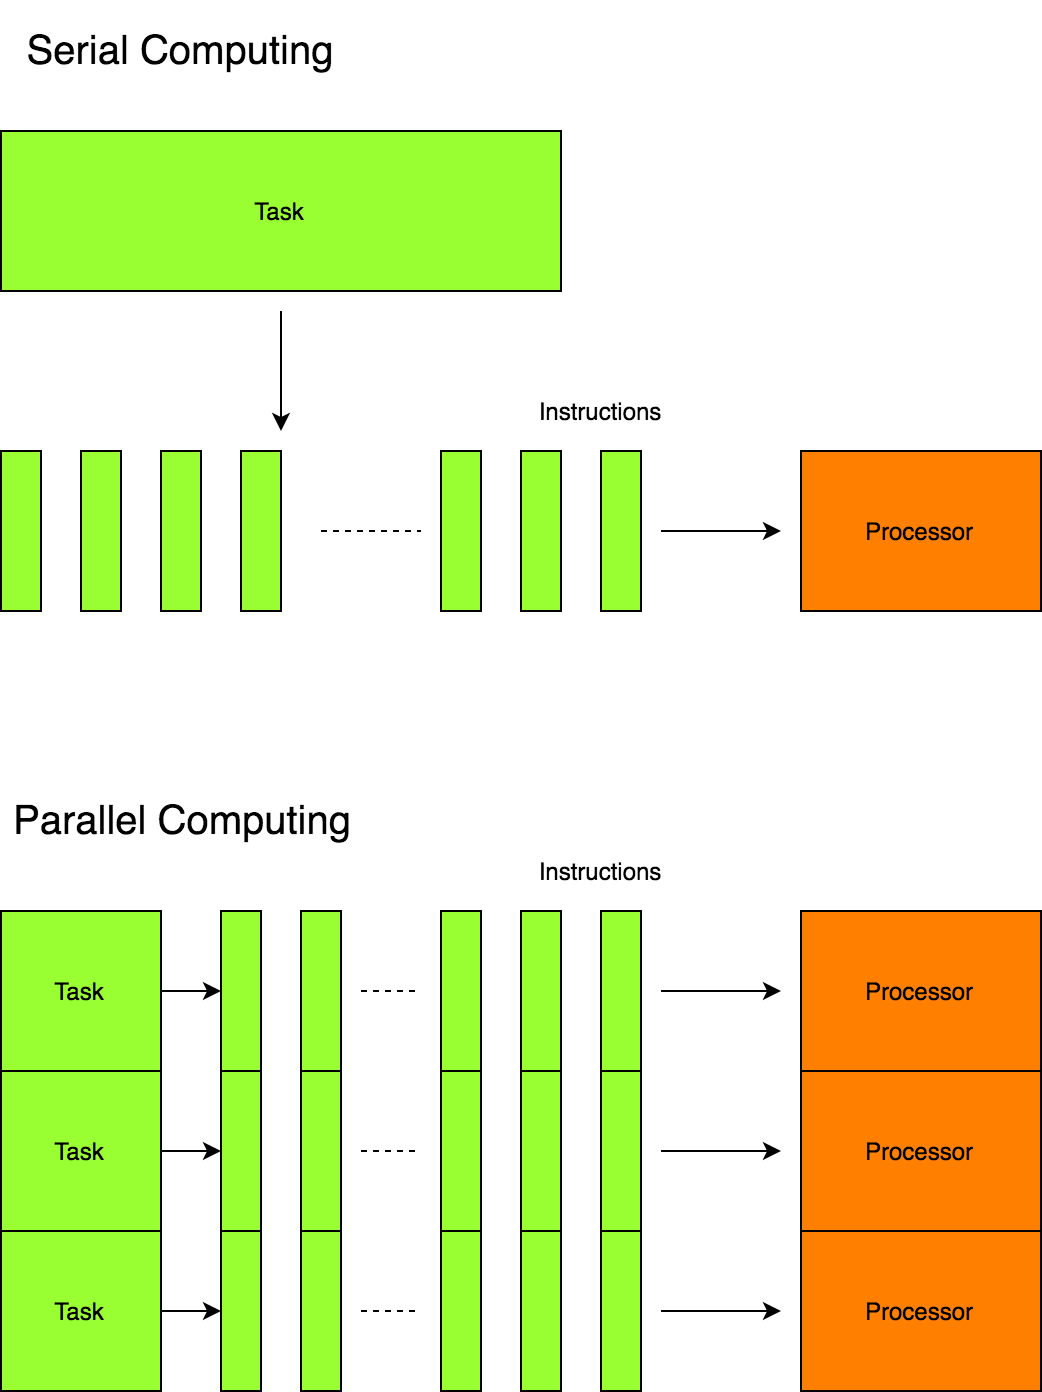
\includegraphics[width=7cm]{Parallel.png}
\centering
\caption{Comparison between Serial and Parallel Computing}
\end{figure}
~\\

\subsection{Motivation}

The drive to utilize parallel computing is strongly related to real world problems, where many events, complementing each other, happen more or less simultaneously, however inside a chronological sequence. Because of how natural phenomena work and how complex they are, serial computing is not suited for heavy workload of modeling and simulation such events. Serialize computation is too time-consuming for this kind of tasks, as being only able to do one job at a time. \\
~\\
Parallel computing, on the other hand, is clearly much more fitted for this line of work. By taking advantage of computers network, whether it is a local or remote one, tapping into parallel potential within modern computer hardwares(multi-core CPU, CUDA GPU) or even both of the above at the same time, parallelization provides the power needed to not only solving mathematical problems with high level of complexity that can be impossible to run on serial computing model, but also gaining better performance time, result in more computation tasks can be done, hence more efficient and profitable. \\


\subsection{Flynn's taxonomy on parallel architecture}

Introduced in 1966, Michael J. Flynn, the author, suggested that high-speed computer can be divided into 4 main categories, based on Instruction Stream and Data Stream. Stream, as Flynn explained (1966), "refers to sequence of data or instructions as seen by the machine during the execution of the program". Flynn clarified further that Instruction Stream and Data Stream serve as a convenient baseline to classify computer organization while preventing any confusion driven by the term "parallelism". \\
\begin{figure}[H]
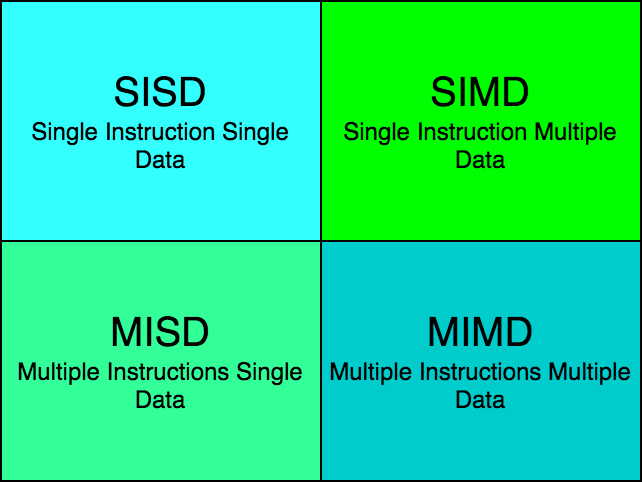
\includegraphics[width=7cm]{Flynn.png}
\centering
\caption{Flynn's taxonomy}
\end{figure}
~\\
%Some images to illustrate this
The computer organization are classified as below:
\begin{itemize}
	\item Single Instruction Stream, Single Data Stream (SISD): Also known as serial (non-parallel) computation, this is the oldest type of computer, in which the processing unit can only take one instruction stream and use one data stream as input at a time during a clock cycle.
	%Image for each kind of architectures
	\item Single Instruction Stream, Multiple Data Stream (SIMD): A popular parallel architecture (appears the most in GPU) that processing units take the same instruction stream during a clock cycle, but the data stream given to them are different from one another. An example of SIMD is image processing, where the processing unit was given one instruction stream to some(or even all) of their core/thread, handling many pixels (multiple data stream) at the same time.
	\item Multiple Instruction Stream, Single Data Stream (MISD): As the opposite of SIMD, this parallel organization is about multiple processors each have its own instruction stream while being fed with a common data stream. However, this kind of architecture is very uncommon compares to the other three.
	\item Multiple Instruction Stream, Multiple Data Stream (MIMD): By far the most common class of parallel computer, especially in modern supercomputers, MIMD allows every processing units can have a different instruction stream and a different data stream. Different tasks can be handled by differnet processors, working on their own set of instructions and data. Because of this, task execution can be either synchronus or asynchronus, depending on the nature of the tasks.
\end{itemize}


\subsection{Maximum performance boost by Parallelization(?)} 
While parallelism can provide better computation time compares to serial computing, there is a limit to how much parallelization can boost performance. Published in 1967, Gene M. Amdahl's paper, "Validity of single processing approach to achieving large scale computing capabilities", stated that there is a boundary in which how parallelism can speed up execution time, given there are always sequential overhead that slow down the computation tine and can't be spedup by applying parallelism. To represent this remark about the speedup, Admdahl gave a the following fomular: \\
\begin{equation}
Speedup = \frac{1}{r_s + \frac{r_p}{N}} \\
\end{equation}
where r$_s$ stands for the serial portion of the code, the overhead that can't be paralleled. $r_p$ describes the parallel part of the program and $r_s + r_p = 1$. N illustrates the number of parallel processors. \\
~\\
In general, this equation implies that the speedup of parallel computing of N processors, compares to serial computing, can never be N times, because of the nature of the overhead as mentioned earlier. More importantly, if N ever reaches infinity, the speedup will equal to $\frac{1}{r_s}$. This number represents the bottle-neck of parallelism and is independent from the number of processors, meaning that the speedup also depends a lot on the program itself, how much of the code can and can't be paralellize. \\

\subsection{Drawbacks of Parallel Computing}
Despite all of its advantages by exploiting the potential of computer resource, both multicore processors and computers network, Parallel Computation, like all things, is not perfect and has can be a double-edge sword. As stated in the previous sections, speedup gained from parallelism does not align with the total number of processors or parallel workflows used in running the program. Because bottle-neck factor comes from the program, it may be redundant to implement parallelism in some cases, where the performance gain might be insignificant, or even loses to serial computing. This is known as parallel slowdown. \\
~\\
Aside from the program's overhead produced by the serial portion of the code, other factors can affect slow down the computation time. Task scheduling plays a major role in this. In reality, for parallelism to function properly, the work needs to be divided and distributed to processors by the task scheduler, which will take time. The more the program has to be splitted, the more time it takes to for task scheduling to complete. Not to mention, more parallel tasks means that it will take more time to communicate between them. If the performance gain from parallel cannot justify these factors, a parallel slowdown is bounded to occur, thus rendering the parallelization useless. \\
~\\
How to implement parallelization is another drawback of this kind of computation. Generally, putting parallelism into practice is rather more complicated than people give it credit for. Not only does the programmer has to deal with the flow of instructions, he also has to take into account the data flow and avoid data dependencies, which agurably is the most problematic part of parallelism, where it is possible. Basically, data dependencies is when data needed from one instruction is related and depends on data of other instructions, thus making that part completely sequential and unparallelable. After successfully implemented parallelism, another challenge is to optimize the parallelization to yield the best possible performance compare to serial computing. \\
~\\
Another disadvantage of parallel computing that should be mentioned is the cost of computer resource. To effectively run paralleled softwares/programs, it usually requires a (or in some cases serveral) multicore CPU, which can be rather expensive, ranging from \$300 to \$1000 for a normal consumers multicore CPU. Higher grade CPU and system for High Perfomance Computing can cost thousands of dollar. Not only CPU can be costly but also dedicate GPUs and Memory as well. However, cost of HPC system is still feasible for many research institutes and individuals compares to supercomputer. \\


\section{Large Scale Parallelism: High Performance Computing system}
High Performance Computing system, or HPC for short, is designed to handle large computation problems, commonly seen in scientific researches, which require strong parallelism performance. An HPC system can comprise of many computers, can be either in the same configuration or different specification from each other. In these machines, there are typically one or multiple Central Processing Units (CPUs), each has multiple processors. In addition, Memory that is much better in term of quality compares to consumer-grade product is installed in these kind of systems to ensure they have the best possible data access time. Moreover, for better parallel capability, computers in HPC system can be equipped with Graphic Processing Units (GPUs), specifically GPUs that support CUDA, a parallel computing platform and application programming interface designed by Nvidia. \\
~\\
Being one of the most powerful and flexible research tools to date, HPC systems are utilized to assist scientists in the study of real world events as mentioned in previous section. While Personal Computers are very powerful on their own and can handle some advanced scientific programs, given that their components are top of their class, they still lack the horse-power needed to solve much heavier mathematical problems. HPC systems, on the other hand, provide the power of many computers combine, usually have better performance than those of Personal Computers, especially in parallel computation, thus accel in that regard. Because of this, HPCs are mostly seen in research institutes, data centers, or just about anywhere that is in need of and benefits from their parallel computational power. \\

\subsection{Cluster Computing System}

Cluster computing system is best described as a combination of stand-alone computers/workstations connected to each other locally via local network or internetwork to act as a single computer. Each machine in the Cluster system is considered as a node, having its own CPUs, whether it is single-core or multi-core, Memory, Network Interface hardware and other components. A cluster usually has 2 or more nodes integrated and can have shared storage for easy data accessing. To exchange data between with each other, nodes are connected to High Performance Network/Switch, for example Gigabit Ethernet, and the Network Interface hardwares are in charge of sending and receiving node's data. Cluster computing is also referred to as High Performance Distributed computing. \\
~\\
% Illustration here
Introduced by IBM in the 1960s as a concept, Cluster computer has exploded into the scene later down the line in the 1980s with the rise of current-time trends: high-performance microprocessors, high-speed network, standard tools for high performance distributed computing, and the increase in performance over price ratio in commodity computers components. As the technology has gotten more advanced as time goes, high-performance computer parts are readily available with fairly affordable price for their power, thus making Cluster computing systems that are built using off-the-shelf components an alternative to supercomputer, becoming an orthodox for high-performance, wide-throughput, readily-available parallel and distributed computing platform. \\

\subsection{Grid Computing System}

Grid computing gives an impression of simple and manageable yet very powerful virtual computer while in fact, Grid is a network of computers coupled together. Unlike Cluster computers, which are locally connected independent computers, Grid Computing systems is a distributed computing infrastructure on a larger scale, not limited to local network or internetwork. Typically, Grid Computation's scale can be of that of geographical, in which each computer system that is part of the grid is placed in a different part of a city, country or even the world. \\
~\\
% Illustration here
Beside the fore-mentioned motivation of the need for parallel performance, Grid Computing also fulfills the purpose of removing the geographic barriers for collaboration on large-scale researches globally with minimum delay. Grid Computing provides means of managing distributed data access, processing data and storage, thus allowing data to be used by wider audiences. Sharing data is not the only thing Grid is capable of but also sharing computation resource, allow users to conduct experiments that are otherwise inefficient and impossible without it. \\


\section{Local Scale Parallelism}

While Large Scale Parallelism system relies on splitting the work and have it done on many computers or processors, may it be single-core or multi-core, Local Scale Parallelism, on the other hand, depends entirely on the nature of the modern multi-core CPU. A multi-core CPU, as the name suggests, consists of 2 or more individual physical processing units, or cores, in one single package. These cores are coupled with each other by connecting to the bus of a shared cache memory within the CPU. Essentially, multicore CPU's architecture is designed following the MIMD architecture. Execution of multiple instructions at once is possible by feeding them into different cores, and each core, as a distinct processing unit, can handle its own set of data different from that of other cores. \\
%image of multi-core parallel
~\\
Current generation multi-core CPU also support what known as thread-level parallelism. This is kind of Local Scale Parallelism that executes tasks on individual threads of the CPU. A thread is basically a distinct process with its own instruction and data, and it can represent a part of a parallel program containing multiple processes. Thread-level parallelism is represented in the form of multithreading, having multiple threads sharing the same functional units of a processor. For this reason, thread-level parallelism will increase computation performance, especially in demanding tasks that require doing multiple tasks at the same time, such as video rendering, which requires both raw computational power and multiple parallel throughputs. \\
%image of thread level parallel
%May be I need a section on Graphic Processing Unit?